\section{Stable Diffusion}
\label{sec:stable_diffusion}


\begin{figure}
    \centering
    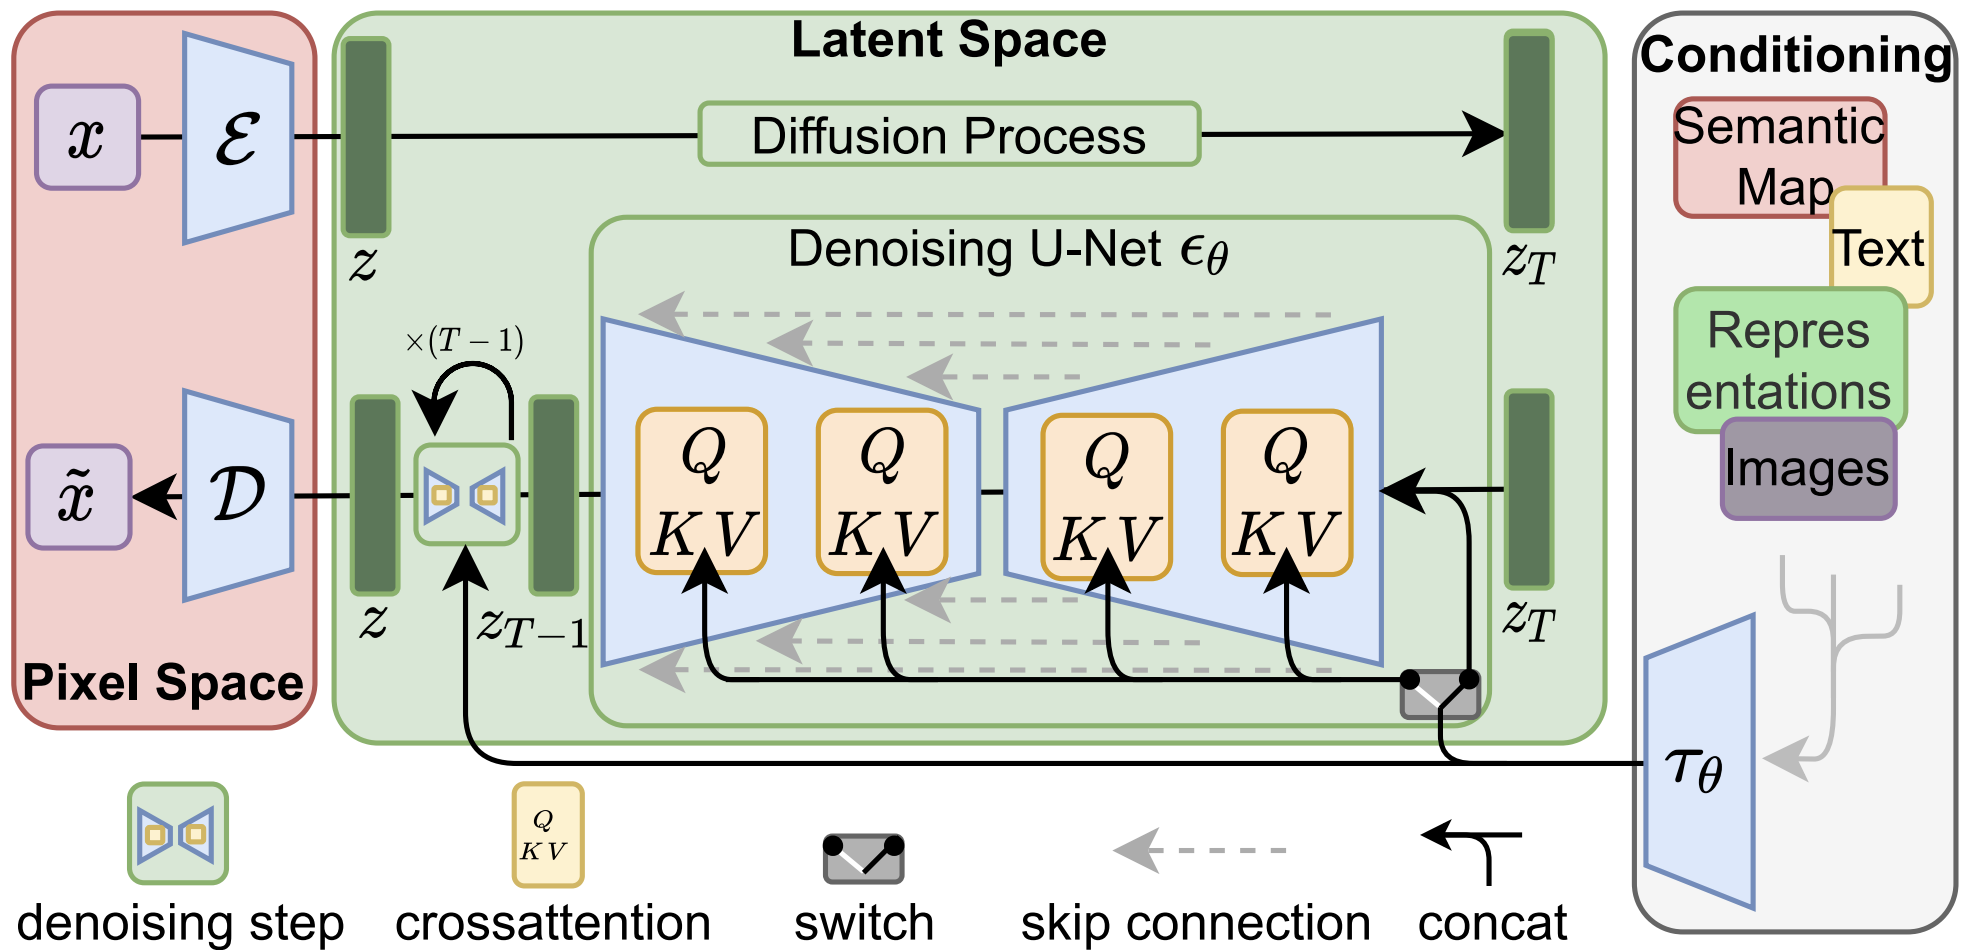
\includegraphics[width=0.8\textwidth]{images/diffusion_models/stable_diffusion/stable_diffusion.png}
    \caption{Stable diffusion scales better compared to other models \cite{stable_diffusion} (DALL-E, VQGAN) with less downsampling blocks (4 instead of 16 as needed by VQGAN).}
\end{figure}


Stable diffusion models are based on latent diffusion. In the paper \cite{stable_diffusion} the authors suggested that computing gradients directly on the pixel space is inefficient, since this space is high-dimentional and includes imperceptible details (high-frequency undesired details). Instead, they suggest to first convert the training images to a lower-dimensional latent space and then apply the diffusion processes on this space. The computation is done on the latent space instead of the pixel space. The authors showed that this approach scales better to higher dimension inputs, and showed significant competitive performance on multiple tasks while lowering significantly computational costs.  And finally, the authors introduced general purpose conditioning mechanism based on cross-attention which allows multi-modal training.

% This process is much more efficient, and in the paper \cite{stable_diffusion} the authors showed that the model can be trained on a single GPU with 16GB of memory. The model is trained on a 256x256 resolution CelebA-HQ dataset with 30 diffusion steps.

% An example of this is when giving an image to a person and asking them to describe the image, they will not describe the individual pixel values, but instead describe the high-level features of the image first.

A 2021 paper released by OpenAI \cite{openai_diffusion_beats_gans} shows that diffusion models can outperform GANs in terms of image fidelity by trading off diversity.














\subsection{U-Net backbone}
\label{subsec:stable_diffusion_u_net_backbone}

U-Net (first introduced in 2015) \cite{unet} is a convolutional neural network architecture that is commonly used in diffusion models, particularly in stable diffusion models and its variants. U-Net is used as a backbone for denoising the latent representations. The U-Net architecture is a symmetric encoder-decoder network with skip connections between the encoder and decoder. The skip connections help the network to learn better (by minimizing \textbf{exploding / vanishing gradient problem} \cite{exploding_vanishing_gradients}), the downsampling process of the encoder removes abstract features in the data, and so skip connections allow the model to skip these downsampling blocks and preserve high-level features. In the original DDPM paper \cite{ddpm} the authors didn't explicitly used U-Net, however they used CNN with residual blocks, which is similar in structure and intent to U-Net. 

\begin{figure}
    \centering
    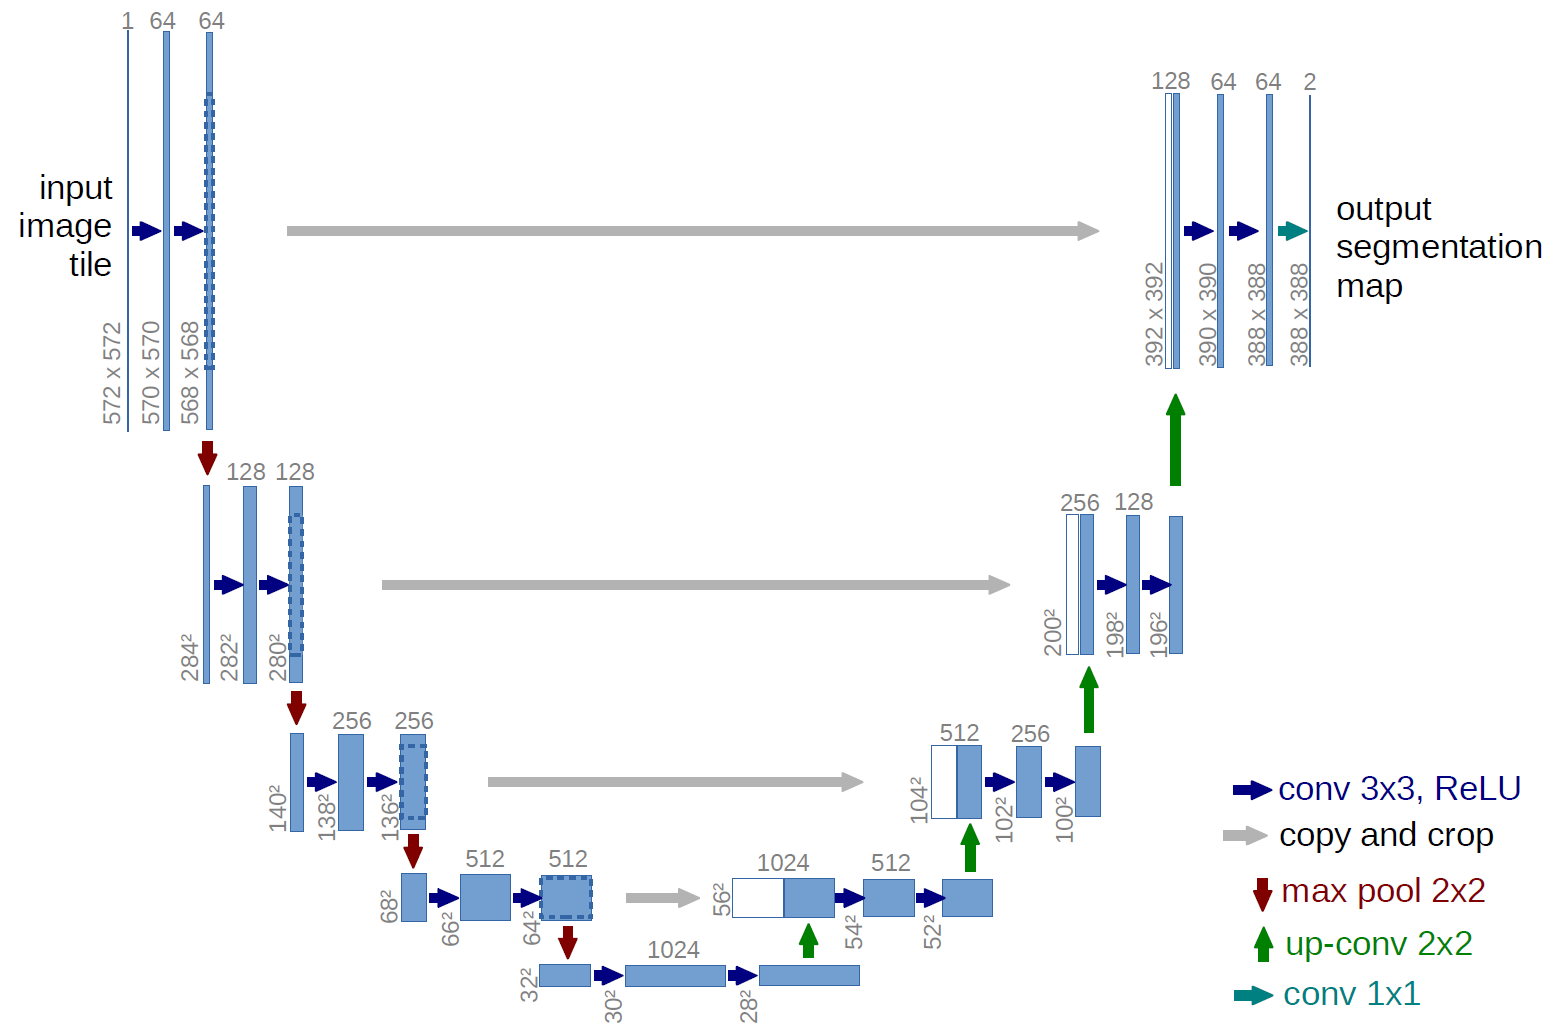
\includegraphics[width=0.8\textwidth]{images/diffusion_models/stable_diffusion/u-net-architecture.png}
    \caption{U-Net architecture \cite{unet}, with convolutional and deconvolutional layers, and skip connections. This architecture is commonly used in stable diffusion models.}
    \label{fig:unet_architecture}
\end{figure}

In figure \ref{fig:unet_architecture} the U-Net is shaped like a 'U' - notice that the layers downsample the input one after the other. Then, after we get to the desired depth, we start upsampling the input until we get output with the same dimensions as the input. The blue arrows are the convolutional layers with kernel size 3x3 and ReLU activation function. The max-pooling are the downsampling layers, and the upsampling layers are the deconvolutional layers.

\subsection{Sinusoidal embeddings}
\label{subsec:sinusoidal_embeddings}

In addition, the UNet backbone contains \textbf{timestep embeddings}. The scalar timestep (which can be in the range $[0, T]$, where $T$ is the total number of diffusion steps) is first projected into a \textbf{sinusoidal embedding}, similar to the way positional encodings are used in transformers. The timestep embeddings are used to let the model know which step its in the diffusion process currently, this way it knows if its in the beginning of the diffusion or at the late stage, which is essential for removing noise.

\begin{figure}[h]
    \centering
    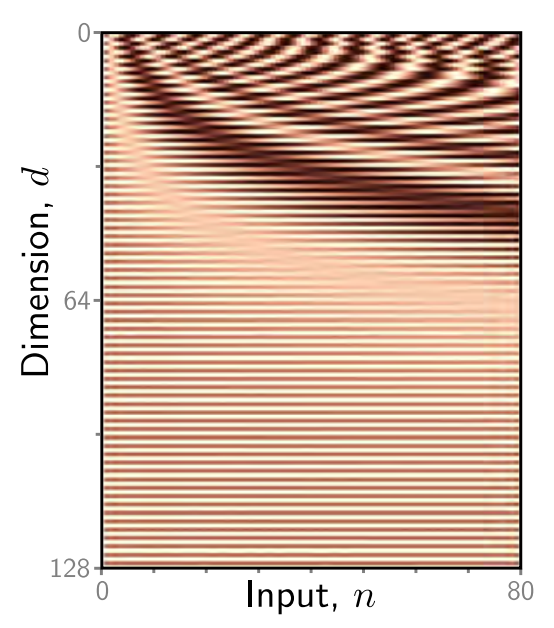
\includegraphics[width=0.25\textwidth]{images/diffusion_models/stable_diffusion/positional_encodings.png}
    \caption{Sinusoidal positional embeddings used in a transformer model \cite{understanding_deep_learning_book_2024}. It is similar to the timestep embeddings used in stable diffusion U-Net backbone. The X axis is the position of the input sequence (or timestep). The Y axis is the embeddings dimensions. The pattern is sinusoidal, lighter regions indicate lower value, darker regions indicate higher values. Its important to note that each column in the X axis is a unique encodings, which helps distinguish the position / timestep of the input sequence.}
\end{figure}

In other words, the U-Net denoises the latent space, and the VAE decoder takes in the denoised latent vectors and generates image based on the latent vectors.

\begin{lstlisting}[language=Python, breaklines=true, caption={Timestep embeddings of Stable Diffusion pipeline. We convert the timestep to sinusoidal vector embedding.}, label={lst:timestep_embeddings_stable_diffusion}]
def get_time_embedding(timestep):
    # Shape: (160,)
    freqs = torch.pow(10000, -torch.arange(start=0, end=160, dtype=torch.float32) / 160) 
    # Shape: (1, 160)
    x = torch.tensor([timestep], dtype=torch.float32)[:, None] * freqs[None]
    # Shape: (1, 160 * 2)
    return torch.cat([torch.cos(x), torch.sin(x)], dim=-1)
\end{lstlisting}

The general formula for timestep embeddings is given in equation \ref{eq:timestep_embeddings}. The code snippet in listing \ref{lst:timestep_embeddings_stable_diffusion} is taken from \href{https://github.com/hkproj/pytorch-stable-diffusion/blob/e0cb06de011787cdf13eed7b4287ad8410491149/sd/pipeline.py#L164}{a re-implementation of Stable Diffusion}.

\begin{equation}
    \text{Enc}_i(t) =
    \begin{cases}
        \sin\left(\frac{t}{10000^{\frac{2i}{d}}}\right) & \text{if } i \text{ is even} \\
        \cos\left(\frac{t}{10000^{\frac{2i}{d}}}\right) & \text{if } i \text{ is odd}
    \end{cases}
    \label{eq:timestep_embeddings}
\end{equation}








\subsection{Architecture}

The stable diffusion model, which is a latent diffusion model (LDM), consists of: variational autoencoder which compresses the input images into regularized latent space as an image encoder, a U-Net backbone which denoises the output from forward diffusion backwards to obtain a latent representation (it predicts the noise added in each step), a variational autoencoder decoder which converts the latent representation back to the image space, and an optional classifier-free guidance mechanism which allows the model to be conditioned on text prompts or other images, which is domain-specific encoder. The high level architecture is shown in figure \ref{fig:stable_diffusion_architecture}.

The most popular conditioning mechanism is text prompts. For text, we use text encoder (tokenizer) which converts the text words to vectors / embeddings (tokens). In Stable Diffusion paper, the authors used a \href{https://github.com/CompVis/latent-diffusion/blob/a506df5756472e2ebaf9078affdde2c4f1502cd4/ldm/modules/encoders/modules.py#L138}{frozen CLIPTokenizer}, which is a pre-trained tokenizer trained on specific vocabulary and special tokens (beginning of sentence, end of sentence, padding, mask tokens and more). Although in the source code you will find other text encoders as well, such as BERT \cite{bert}.

\begin{figure}
    \centering
    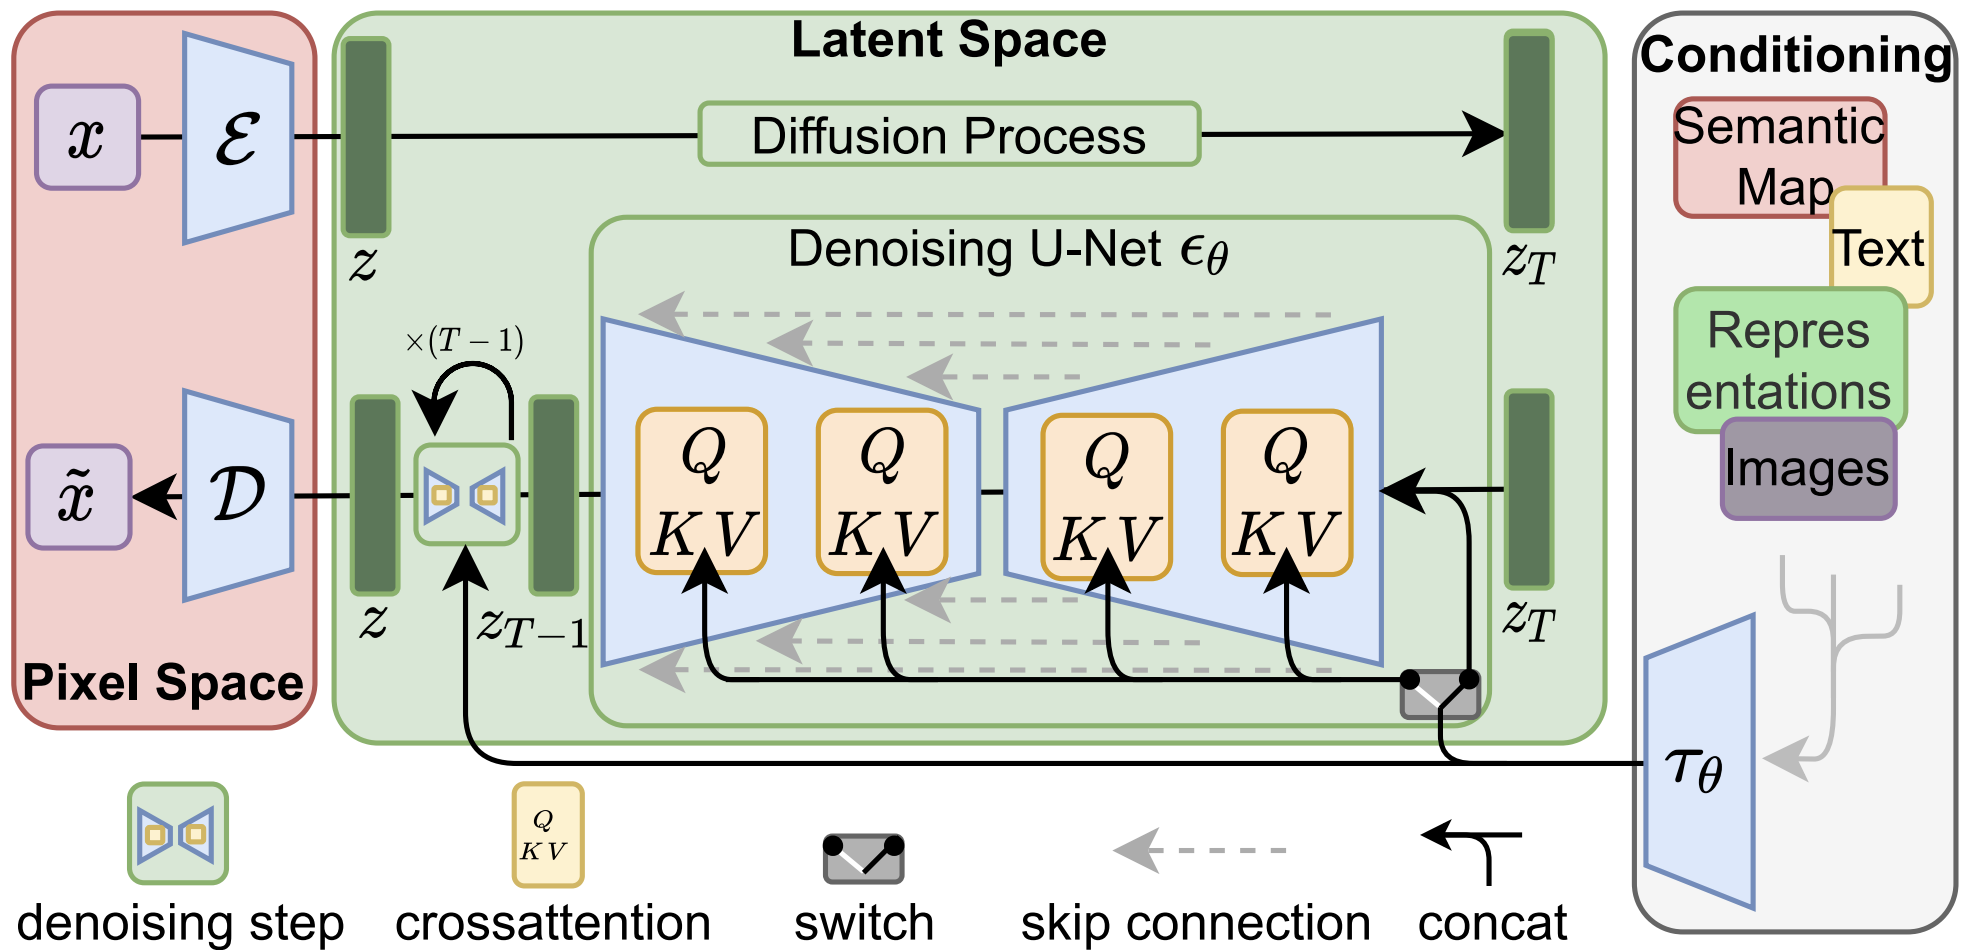
\includegraphics[width=0.75\textwidth]{images/diffusion_models/stable_diffusion/architecture.png}
    \caption{Stable diffusion architecture \cite{stable_diffusion}. The 'switch' in the diagram is used for different applications of conditional information. In the case of text, they use cross-attention. If the conditional information is spatial (such as images, layouts, semantic masks), they use concatenation.}
    \label{fig:stable_diffusion_architecture}
\end{figure}

How the model is able to denoise latent space but also consider the conditional information? The authors used \textbf{cross-attention} mechanism. The cross-attention which was introduced in the transformers paper \cite{transformer}, is a mechanism that allows the model to focus on different parts of the input sequence. In the stable diffusion model, the cross-attention mechanism is used to focus on the latent space and the conditioning signal (text prompt or another image). 

The U-Net architecture, which serves as the noise prediction network, incorporates timestep embeddings as an essential input (see \ref{subsec:stable_diffusion_u_net_backbone}). These timestep embeddings, combined with residual blocks, allow the U-Net to predict the noise at each timestep of the diffusion process. This prediction is not only dependent on the specific timestep but also conditioned on the given conditional signal. 











\subsection{Classifier-free diffusion guidance (CFG)}

\label{subsec:classifier_free_diffusion_guidance}

So far we have focused on modeling just the data distribution $p(x)$. However, we are often also interested in learning conditional distribution $p(x|y)$, which would enable us to explicitly control the data we generate through conditioning information $y$.

We can add conditioning information alongside the timestep information, at each iteration:

\[
p(x_{0:T}) = p(x_T) \prod_{t=1}^{T} p_\theta (x_{t-1} | x_{t, y})
\]

When training a diffusion model to generate images based on specific conditional information, there's a risk that the model might not fully consider or even ignore these conditions, using this vanilla formulation. To address this, a technique called "guidance" is used. Guidance allows us to explicitly control how much influence the conditions have on the generated images, but this can sometimes lead to less variety in the results. In other words, we use weight to control how much the model should pay attention to the conditioning signal.

Conditioning a generative model can be achieved through various methods. One method called \textbf{classifier guidance} \cite{openai_diffusion_beats_gans} \cite{score_based_generative_modeling} \cite{openai_diffusion_beats_gans}, which involves training a separate model to condition the output, and is based on \textbf{score-based diffusion models} \cite{score_based_generative_modeling} (which is out of the scope of this paper). In short, classifier guidance formulation is given as:

\[
\nabla \log p(x_t | y) = \underbrace{\nabla \log p(x_t)}_{\text{unconditional score}} + \underbrace{\gamma \nabla \log p(y | x_t)}_{\text{adversarial gradient}}
\]

where $\gamma$ is a hyperparameter that controls the strength of the conditioning signal in classifier guidance method.

Another guidance approach, which is the latest and most successful approach, is called \textbf{classifier-free guidance} \cite{classifier_free_guidance} (CFG), in which, instead of training two networks, one conditional network and an unconditional network, we train a single network and during training, with some probability, we set the conditioning signal to zero. This way the network becomes a mix of conditioned and unconditioned network, and we can take the conditioned and unconditioned output and combine them with weight that indicates how much we want the network to pay attention to the conditioning signal. In other words, we control the weight of the conditioning signal during training. The formulation for classifier-free guidance is given by:

\[
\nabla \log p(x_t | y) = \underbrace{\gamma \nabla \log p(x_t | y)}_{\text{conditional score}} + \underbrace{(1 - \gamma) \nabla \log p(x_t)}_{\text{unconditional score}}
\]

To summorize, in contrast to classifier guidance, classifier-free guidance streamlines the training process and lowers computational costs by utilizing a single model instead of training two separate models.

\begin{lstlisting}[language=Python, caption={Classifier-free guidance (CFG) in Stable Diffusion. The CFG scale is the weight of the conditioning signal.}, label={lst:cfg_stable_diffusion}]
if do_cfg:
    output_cond, output_uncond = model_output.chunk(2)
    model_output = cfg_scale * (output_cond - output_uncond) + output_uncond
\end{lstlisting}

In listing \ref{lst:cfg_stable_diffusion} the code snippet is taken from \href{https://github.com/hkproj/pytorch-stable-diffusion/blob/e0cb06de011787cdf13eed7b4287ad8410491149/sd/pipeline.py#L135C1-L136C1}{a re-implementation of Stable Diffusion}, but the official implementation of Stable Diffusion is \href{https://github.com/CompVis/stable-diffusion/blob/21f890f9da3cfbeaba8e2ac3c425ee9e998d5229/ldm/models/diffusion/ddim.py#L178C1-L179C1}{very similar}.

















\subsection{Contrastive Language Image Pre-training (CLIP)}

\label{subsec:clip}

In Stable Diffusion, the authors used CLIP as the text encoder for the conditional information of text prompts.

CLIP (Contrastive Language Image Pre-training) \cite{openai_clip} is a model developed by OpenAI that learns visual concepts from text supervision. The model builds associations between images and text prompts. Often this association is called 'text-image alignment', or 'image-text alignment'. It models how well a generated image corresponds to its associated text description.

This is why the researchers use the \textbf{CLIPTokenizer} which is part of the CLIP model. This tokenizer converts text prompts to a sequence of tokens which are then used in the latent space of the stable diffusion model. They use the embeddings of this pre-trained model.

\begin{figure}
    \centering
    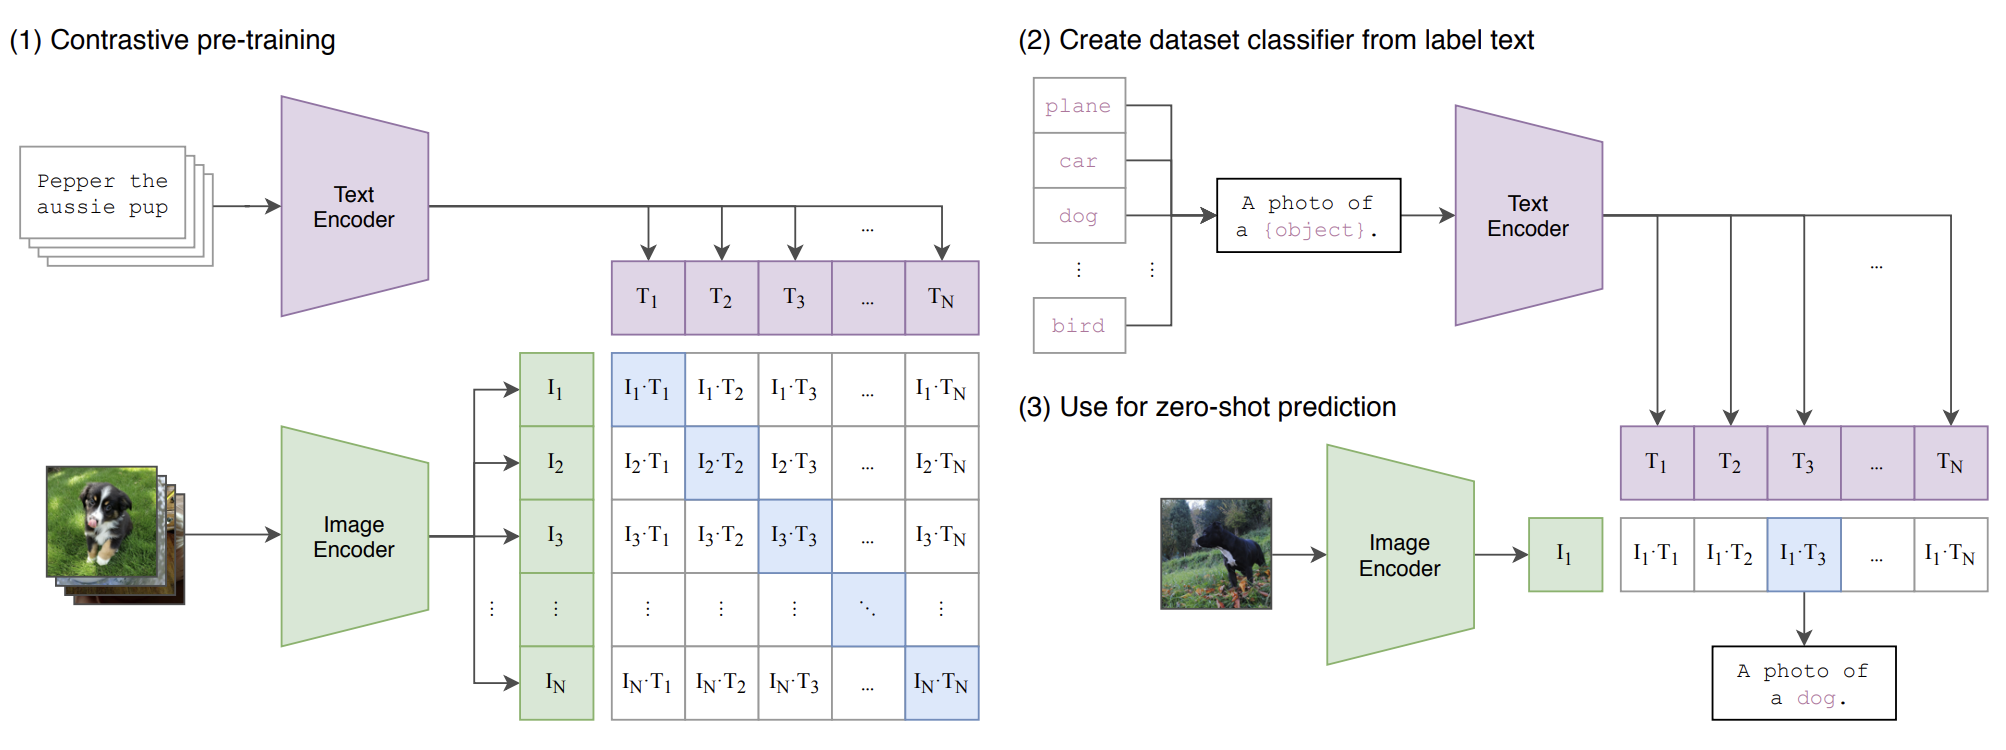
\includegraphics[width=1\textwidth]{images/diffusion_models/stable_diffusion/clip.png}
    \caption{(1) Contrastive pre-training stage of a CLIP model \cite{openai_clip} (training stage). The $I_1, ..., I_N$ are the images, and $T_1, ..., T_N$ are the text prompts. The output is a matrix of similarity scores between the images and the text prompts. (2) and (3) after the model is pre-trained its used as a zero-shot image classifier (the model can classify images without needing to be explicitly trained on specific classes).}
    \label{fig:openai_clip}
\end{figure}

In figure \ref{fig:openai_clip}, the diagonal of the similarity matrix ideally contains the highest scores for matching image-text pairs (idealy '1'), while the off-diagonal entries should have lower similarity scores (idealy '0'), indicating mismatches between images and texts.

The network implementation of CLIP is made up of an image encoder, which is typically a vision transformer (ViT) \cite{vision_transformer} or sometimes less commonly a ResNet \cite{resnet} model, while the text encoder is a text transformer \cite{transformer} or continous bag of words \cite{cbow_word2vec} (more commonly known as Word2Vec model by Google, 2013).

The CLIP model is trained using a contrastive objective, where the goal is to minimize the cosine distance between embeddings of matching image-text pairs (diagonal) and maximize the distance for non-matching pairs (off diagonal). Just like in word2vec, the training process also needs to include negative examples of images and captions that don't match, and the model needs to assign them low similarity scores.














\subsection{Cross-attention}
\label{subsec:cross_attention}

Cross-attention (appendix \ref{appendix:attention}) is used in Stable Diffusion for \textbf{multi-modal conditioning}, it guides the model to output images based on conditional information. Although this information can be multi-modal embeddings (images, text, segmentation masks), the cross-attention mechanism is able to deal with them all.

Cross-attention, introduced in the Transformer paper \cite{transformer}, allows one set of inputs (query vectors) to attend (focus) on another set of inputs (the key vectors) and extract information from it (the value). This is particularly useful in tasks where we want to condition one type of data on another, such as in image-text models (like Stable Diffusion) where text guides the generation of images.

To understand cross-attention lets first understand \textbf{self-attention} (appendix \ref{appendix:attention}):

In self-attention, the same set of data elements provides the queries, keys, and values. The mechanism computes attention scores based on how each element in the input interacts with other elements in the same sequence. This is widely used in transformers to capture relationships between tokens in a sequence. The formula for self-attention is given in the transformer paper \cite{transformer}.

\begin{equation}
    \text{Attention}(Q, K, V) = \text{softmax} \left( \frac{QK^T}{\sqrt{d_k}} \right) V
    \label{eq:self_attention}
\end{equation}

In equation \ref{eq:self_attention} we first do a cross-product of $Q$ and $K$ matrices, this gives us a matrix of attention scores for each pair of query vector and the key vector. We then divide the matrix by the square root of the dimension of the key vectors, this operation is done to normalize the large magnitude of the dot product, which stabilizes the gradients and the training. We then apply the softmax function, which converts the vector to a probability distribution between 0 and 1, which gives probability to tokens in the sequence. Finally, we multiply (dot product) the softmax output with the value vectors, which gives us the output of the self-attention.

\textbf{Cross-attention} (appendix \ref{appendix:attention}) is similar to self-attention, but instead of attending to the same sequence, it attends to a different sequence. In our case, conditional embeddings with the latent vector space of the diffusion model. The cross-attention mechanism is used to focus on the latent space (the output of the encoder) and the conditioning signal (text prompt or another image). Although cross-attention can be used in similar fashion to self-attention, its often used in \textbf{multi-head attention} fashion, where multiple self-attention heads are concatenated together to form a cross-attention mechanism.

The researchers used cross-attention mechanism because of the multi-modal conditioning signals with attention to the latent vector.

\begin{equation}
    \begin{aligned}
        \text{head}_i = \text{Attention}(QW_i^Q, KW_i^K, VW_i^V)  \\
        \text{MultiHead}(Q, K, V) = \text{Concat}(\text{head}_1, ..., \text{head}_h)W^O
    \end{aligned}
    \label{eq:stable_diffusion_multihead_crossattention}
\end{equation}

Formula \ref{eq:stable_diffusion_multihead_crossattention} describes a single self-attention head. Cross-attention is a concatenation of multiple self-attention heads, each with its own set of weights $W_i^Q$, $W_i^K$, $W_i^V$. The output of the cross-attention is the concatenation of the outputs of each head, and dot product with the output weights matrix $W^O$.



\begin{lstlisting}[language=Python, caption={Cross-attention PyTorch code snippet. The '@' operation is a dot product.}, label={lst:stable_diffusion_cross_attention}]
class CrossAttention(nn.Module):
def __init__(self, n_heads, d_embed, d_cross, 
        in_proj_bias=True, out_proj_bias=True):

    super().__init__()
    self.q_proj   = nn.Linear(d_embed, d_embed, bias=in_proj_bias)
    self.k_proj   = nn.Linear(d_cross, d_embed, bias=in_proj_bias)
    self.v_proj   = nn.Linear(d_cross, d_embed, bias=in_proj_bias)
    self.out_proj = nn.Linear(d_embed, d_embed, bias=out_proj_bias)
    self.n_heads = n_heads
    self.d_head = d_embed // n_heads

def forward(self, x, y):
    # ...

    weight = q @ k.transpose(-1, -2)
    weight /= math.sqrt(self.d_head)
    weight = F.softmax(weight, dim=-1)
    output = weight @ v

    output = output.transpose(1, 2).contiguous()
    output = output.view(input_shape)
    output = self.out_proj(output)
    return output
\end{lstlisting}

In listing \ref{lst:stable_diffusion_cross_attention} the code snippet is taken from \href{https://github.com/hkproj/pytorch-stable-diffusion/blob/e0cb06de011787cdf13eed7b4287ad8410491149/sd/attention.py#L100C1-L110C28}{a re-implementation of Stable Diffusion}, the official implementation of Stable Diffusion has \href{https://github.com/CompVis/stable-diffusion/blob/21f890f9da3cfbeaba8e2ac3c425ee9e998d5229/ldm/modules/attention.py#L152}{very complex cross-attention code}.

















\subsection{DDIM Sampler}

\begin{figure}
    \centering
    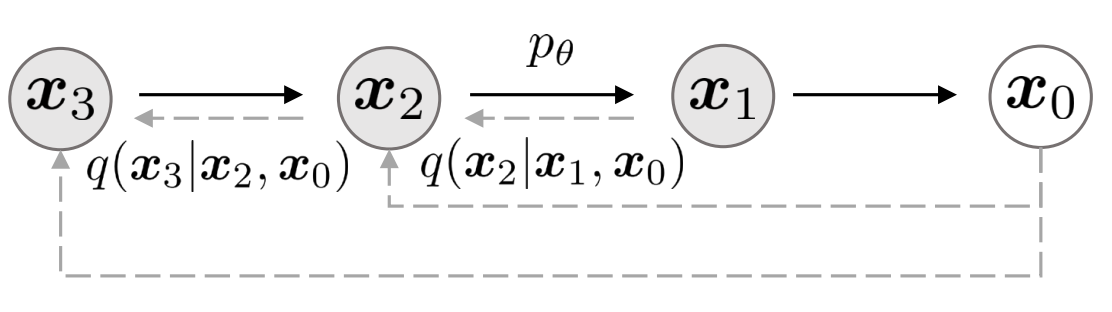
\includegraphics[width=0.8\textwidth]{images/diffusion_models/stable_diffusion/ddim_non_markov_process.png}
    \caption{Non-markovian inference model \cite{ddim} (denoising diffusion implicit models (DDIM) sampler). Each step not only depends on the previous step, but also on the initial step $x_0$.}
    \label{fig:ddim_non_markov_process}
\end{figure}

DDIM (Denoising Diffusion Implicit Models) (intoduced in a 2020 paper by Stanford) \cite{ddim} is a sampling method for diffusion models that offers improvements over the traditional DDPM (Denoising Diffusion Probabilistic Models) \cite{ddpm} approach. Unlike DDPM, which relies on a fixed noise schedule, DDIM introduces a more flexible noise schedule that allows for varying degrees of noise at different diffusion steps. This flexibility can lead to higher-quality and more diverse generated samples. Additionally, DDIM employs a more efficient sampling process, which can result in faster inference times.

In DDPM, images are generated by starting from pure noise and denoising it step-by-step through a Markovian chain (appendix \ref{appendix:markov_chains}). Each step adds a bit of noise to maintain probabilistic reversibility. This process is slow (10x to 50x times slower \cite{ddim}) and often requires hundreds to thousands (1000 steps in the case of Stable Diffusion \cite{stable_diffusion}) of denoising steps to generate a high-quality image. DDIM modifies the denoising process by introducing a \textbf{non-Markovian deterministic sampler} (figure \ref{fig:ddim_non_markov_process}). Instead of stochastically adding noise at each step, DDIM removes noise in a direct and controlled manner, skipping unnecessary steps and resulting in a deterministic path through the latent space.

In DDIM, the reverse process (denoising) can be viewed as solving an ordinary differential equation (ODE) in the latent space. DDIM simplifies the reverse process by computing intermediate noise-free latent variables without adding extra randomness.

To achieve this the researchers introduced a new family of forward process:

\begin{equation*}
    q_\sigma (x_{t-1} | x_t, x_0) = \mathcal{N} (\sqrt{\alpha_{t-1}} x_0 + \sqrt{1 - \alpha_{t-1} - \sigma_t^2} \cdot \frac{x_t - \sqrt{\alpha_t} x_0}{\sqrt{1 - \alpha_t}}, \sigma_t^2 I)
\end{equation*}

where $\sigma$ is a vector of indexes (of the steps): $\sigma \in \mathbb{R}^T_{\geq 0}$. The magnitude of $\sigma$ controls how stochastic the forward process is; when $\sigma \rightarrow 0$, we reach an extreme case where as long as we observe $x_0$ and $x_t$ for some $t$, then $x_{t-1}$ become known and fixed.

% The distribution of $x_t$ is defined given $x_{t-1}$ and $x_0$ - the process is not longer markovian (this equation is derived from Bayes' rule, its also proven that this is also Gaussian distribution):

% \begin{equation*}
%     q_\sigma (x_t | x_{t-1}, x_0) = \frac{q_\sigma (x_{t-1} | x_t, x_0) q_\sigma (x_t | x_0)}{q_\sigma (x_{t-1} | x_0)}
% \end{equation*}

% Now in order to adapt to the reverse diffusion process (which is the entire goal of this paper, to skip intermediate steps of the sampling process), we define this process on the subset $\{ x_{\tau_1}, ..., x_{\tau_S} \}$:

% \begin{equation}
%     p_\theta (x_{0:T}) := p_\theta (x_T) \prod_{i=1}^{S} p_\theta^{(\tau_i)} (x_{\tau_{i-1}} | x_{\tau_i}) \times \prod_{t \in \bar{\tau}} p_\theta^{(t)} (x_0 | x_t)
%     \label{eq:ddim_reverse_diffusion}
% \end{equation}

\begin{figure}
    \centering
    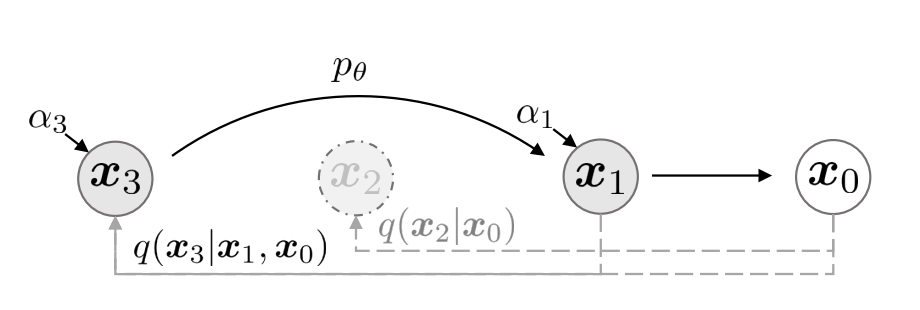
\includegraphics[width=0.8\textwidth]{images/diffusion_models/stable_diffusion/ddim_sampling_process.png}
    \caption{Reverse diffusion process of the DDIM sampler \cite{ddim} for accelerated generation of images. Here we see that $x_3$ depends only on $x_1$ (and not $x_2$) and $x_0$. This process can be generalized to all subsets of steps.}
    \label{fig:ddim_sampling_process}
\end{figure}

\begin{figure}
    \centering
    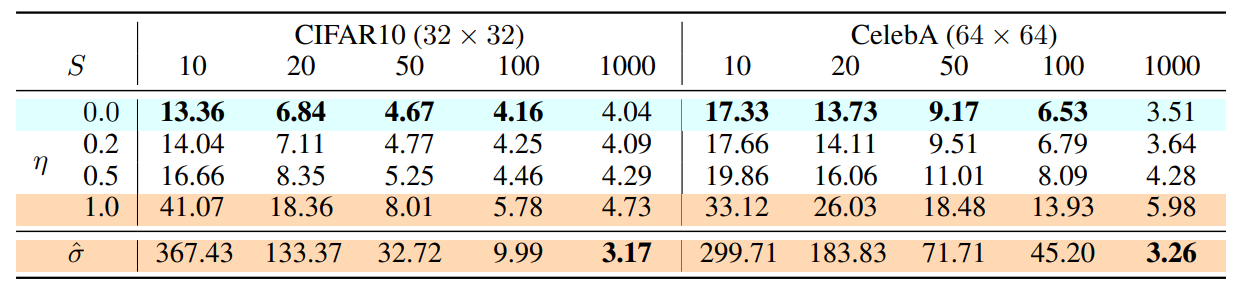
\includegraphics[width=0.8\textwidth]{images/diffusion_models/stable_diffusion/ddim_sample_quality.png}
    \caption{The researchers showed that using this non-Markovian process gives almost the same sample quality (in FID metric eq. \ref{eq:fid_score}, lower is better) as regular DDPM but much less computational cost (since we skip all the latent steps). In the figure, the researchers conducted experiments on CIFAR10 and CelebA datasets, with 10,20,50,100,1000 steps. The stochasticity of the model is controlled by $\eta$. When $\eta = 0$ (blue) the model is deterministic (DDIM process), and when $\eta = 1$ (orange) the model is stochastic (DDPM process).}
\end{figure}

\begin{figure}
    \centering
    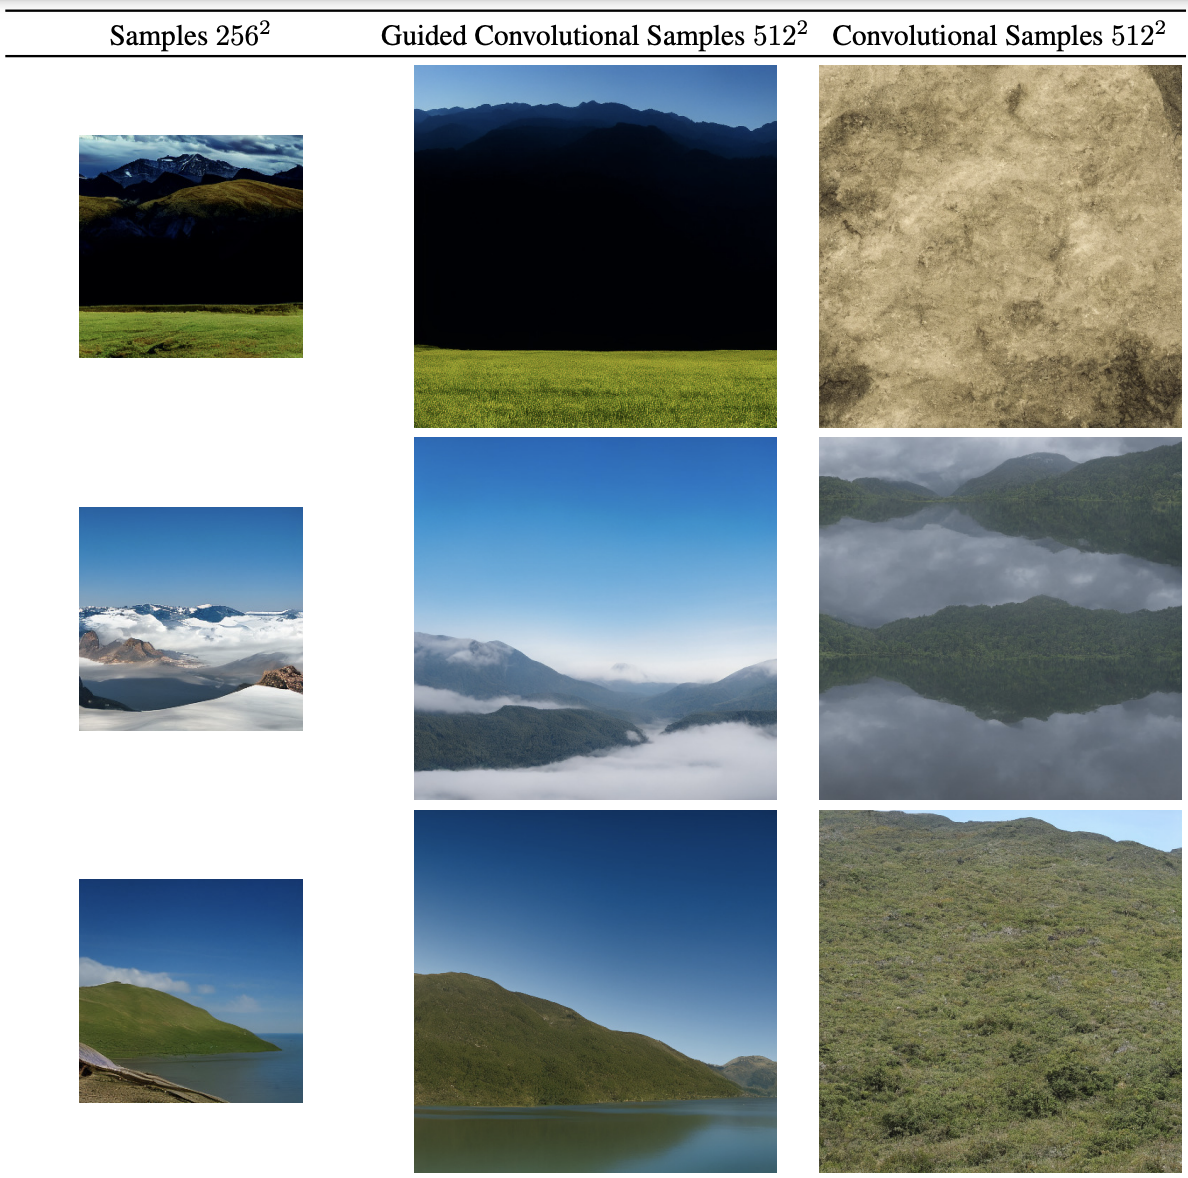
\includegraphics[width=0.8\textwidth]{images/diffusion_models/stable_diffusion/guided_conditioning.png}
    \caption{Guided and unguided conditioning on landscapes dataset. Unguided sampling can lead to incoherent global structures.}
\end{figure}

To summorize, in the DDIM paper \cite{ddim} the main contributions are:

\begin{itemize}
    \item \textbf{Non-markovian diffusion process:} they introduced a new family of forward processes that are non-Markovian, which allows for a more efficient reverse process.
    \item \textbf{Implicit probabilistic model:} DDIM is an implicit probabilistic model, meaning that it does not directly model the joint distribution of the data but rather models the conditional distribution of the data given the noise. This approach allows for efficient inference and faster sampling.
    \item \textbf{Training objective:} DDIM uses the same training objective as DDPM, no modifications needed. This is a huge benefit, because DDIM sampling can be used in any diffusion model.
    \item \textbf{Sampling process:} the sampling process in DDIM involves sampling from the prior distribution and then iteratively sampling from the conditional distributions. This process is faster than traditional diffusion models because it does not require simulating the entire Markov chain.
\end{itemize}
















\subsection{Training}

Stable diffusion uses two-stage approach, called classifier-free guidance (see section \ref{subsec:classifier_free_diffusion_guidance}) which was discuessed before. In the paper the authors made simplified loss objective, which is to predict the noise removal process at each step:

\[
    L_{\text{DM}} = \mathbb{E}_{x, \epsilon \sim \mathcal{N} (0, 1), t} \left[ \Vert \epsilon - \epsilon_\theta(x_t, t) \Vert _2^2 \right]
\]

this loss function is similar to the loss function of DDPM (eqaution \ref{eq:ddpm_loss}).













\subsection{Implementation of $\tau_\theta$ transformer for conditional LDMs}

The researchers provded high level overview of the implementation of the conditional encoder for text $\tau_\theta$, consisted of $N$ transformer blocks:

\begin{align*}
    &\zeta \leftarrow \text{TokEmb}(y) + \text{PosEmb}(y) \\
    &\text{for } i = 1, \ldots, N : \\
        &\hspace{1cm} \zeta_1 \leftarrow \text{LayerNorm}(\zeta) \\
        &\hspace{1cm} \zeta_2 \leftarrow \text{MultiHeadSelfAttention}(\zeta_1) + \zeta \\
        &\hspace{1cm} \zeta_3 \leftarrow \text{LayerNorm}(\zeta_2) \\
        &\hspace{1cm} \zeta \leftarrow \text{MLP}(\zeta_3) + \zeta_2 \\
    &\zeta \leftarrow \text{LayerNorm}(\zeta)
\end{align*}

where $\zeta := \tau_\theta(y)$ is the unmasked transformer output (the transformer processes the tokenized version of $y$), TokEmb is the token embeddings, PosEmb is the positional embeddings, LayerNorm is the layer normalization, MultiHeadSelfAttention is the self-attention mechanism, and MLP is the multi-layer perceptron. The $\zeta$ is the output of the transformer encoder, which is then used in the cross-attention mechanism of the stable diffusion model.

\begin{figure}[h]
    \centering
    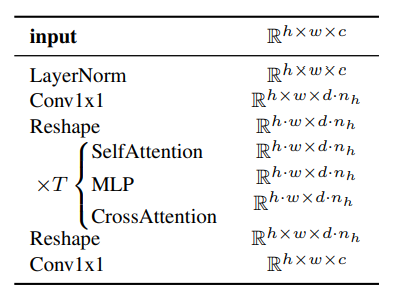
\includegraphics[width=0.4\textwidth]{images/diffusion_models/stable_diffusion/transformer_block.png}
    \caption{Architecture of transformer block, where $n_h$ denotes the number of attention heads and $d$ the dimensionality per head.}
\end{figure}







\subsection{Details on Autoencoders Models}

In the paper, the researchers trained all their autoencoder models (as the image encoder $\varepsilon$, and image decoder $\mathcal{D}$) in adversarial manner (adversarial loss) \cite{vqgan}, such that patch-based discriminator $D_\psi$ is optimized to differentiate original images from reconstructed images $\mathcal{D} (\varepsilon (x))$.

The researchers used two methods for regularization on the latent space:

\begin{itemize}
    \item \textbf{KL-divergence regularization:} similar to variational autoencoders, where the latent space is encoded as a distribution over the data, the KL regularization objective pushes the latent space to be close to a standard normal distribution.
    \item \textbf{VQ regularization:} as we saw in VQ-GAN and VQ-VAE (sections \ref{sec:vqgan} and \ref{sec:vqvae}), the vector quantization regularization forces the latent space to be discrete, which can help the model to learn better by using a codebook $\mathcal{Z}$.
\end{itemize}

They used these regularization in small amount, in KL regularization, they factorized the KL term by a factor of $\sim 10^{-6}$, and in the case of VQ regularization, they used a big codebook (high dimensionality). Its done to obtain high-fidelity reconstructions.

The full loss objective to train the autoencoder model $(\varepsilon, \mathcal{D})$ is given by:

\begin{equation*}
    L_{\text{Autoencoder}} = \min_{\varepsilon, \mathcal{D}} \max_{\psi} \left( L_{\text{rec}} (x, \mathcal{D} (\varepsilon (x))) - L_{\text{adv}} (\mathcal{D} \varepsilon (x)) + \log \mathcal{D}_\psi (x) + L_{\text{reg}} (x; \varepsilon, \mathcal{D}) \right)
\end{equation*}





\subsection{Experiments}

The researchers conducted several experiments with different LDM downsampling factors, and compared the results with other state-of-the-art models (DALL-E, VQGAN, StyleGAN, ProjectedGAN, CogView, GLIDE, and others).

\begin{figure}
    \centering
    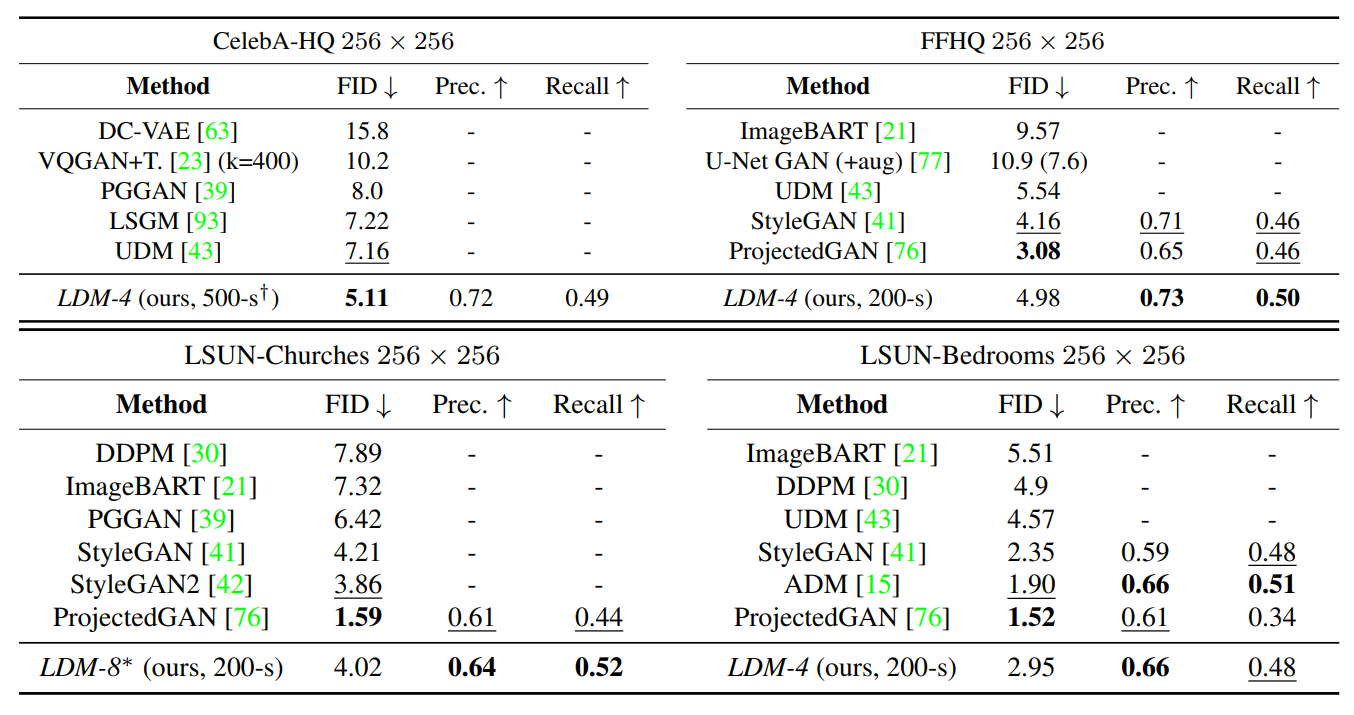
\includegraphics[width=0.8\textwidth]{images/diffusion_models/stable_diffusion/experiments_1.png}
    \caption{Evaluation metrics (FID, Precision, Recall) of unconditional image synthesis between LDM (Stable Diffusion) and other models, across 4 datasets (CelebA-HQ, FFHQ, LSUN-Churches, LSUN-Bedrooms). We clearly see that LDM outperforms most of the state-of-the-art models, across multiple metrics and datasets. $\dagger$ refers to the DDIM sampler steps (500 top-left, 200 top-right, 200 bottom-left, 200 bottom-right).}
\end{figure}

\begin{figure}
    \centering
    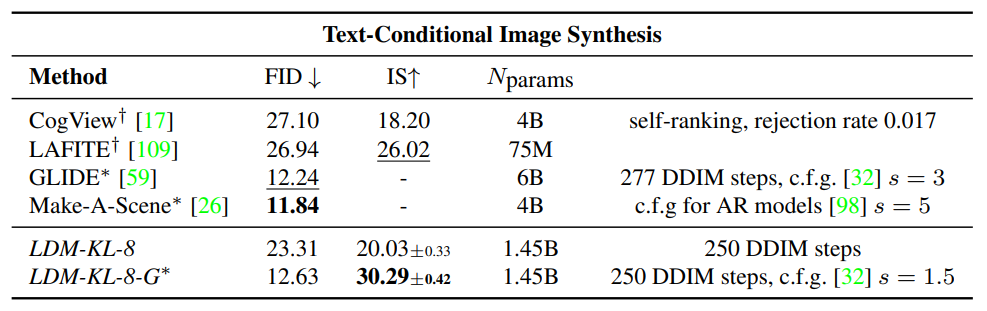
\includegraphics[width=0.8\textwidth]{images/diffusion_models/stable_diffusion/experiments_2.png}
    \caption{Evaluation of text-conditioned image synthesis on MS-COCO dataset. LDM with 250-DDIM steps is on par with the most recent diffusion and autoregressive methods, \textbf{while using significantly less parameters} (1.45 billion).}
\end{figure}

For text-to-image tasks, the researchers trained a 1.45B parameters model conditioned on language prompts on LAION-400M dataset. The model uses \textbf{BERT-Tokenizer} \footnote{Its important to note that the researchers used the BERT text tokenizer in the paper, however, in the \href{https://github.com/CompVis/latent-diffusion}{offical released implementation of Stable Diffusion} they used CLIP tokenizer. The reason is that in the Imagen paper \cite{imagen}, the researchers found out that using larger language models had more impact on generated image quality than larger image generation components. This fact is shown in figure \ref{fig:imagen_clip_score_bigger_llm}.} \cite{bert} and implement $\tau_\theta$ (the domain-specific conditional encoder) as a transformer.

\begin{figure}
    \centering
    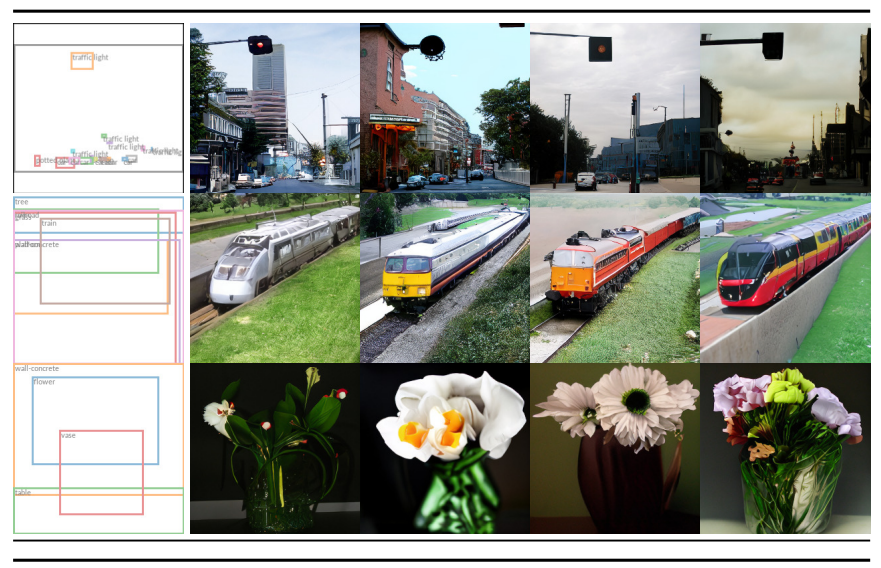
\includegraphics[width=0.8\textwidth]{images/diffusion_models/stable_diffusion/experiments_3.png}
    \caption{Image synthesis conditioned on layouts. The model is trained on OpenImages dataset and then finetuned on COCO dataset.}
    \label{fig:stable_diffusion_experiments_semantic_layouts}
\end{figure}

For semantic layouts, the model is trained to synthesis images based on semantic layouts from the OpenImages dataset and finetune on COCO dataset (see figure \ref{fig:stable_diffusion_experiments_semantic_layouts}).

% \begin{figure}
%     \centering
%     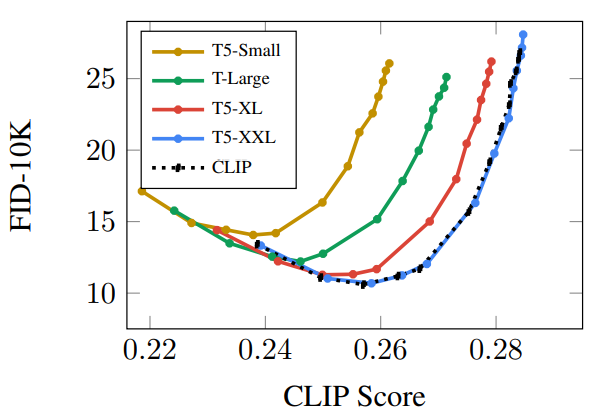
\includegraphics[width=0.5\textwidth]{images/diffusion_models/stable_diffusion/imagen_clip_score_bigger_llm_encoder.png}
%     \caption{Imagen paper \cite{imagen} shows that using larger language models as the text encoder (as conditioning mechanism) has more impact on generated image quality than larger image generation components. This is why in Stable Diffusion, the implementation uses CLIP tokenizer instead of BERT tokenizer (which was used in the paper, originally).}
%     \label{fig:imagen_clip_score_bigger_llm}
% \end{figure}



\begin{figure}[h]
    \centering
    \begin{subfigure}[b]{0.4\textwidth}
        \centering
        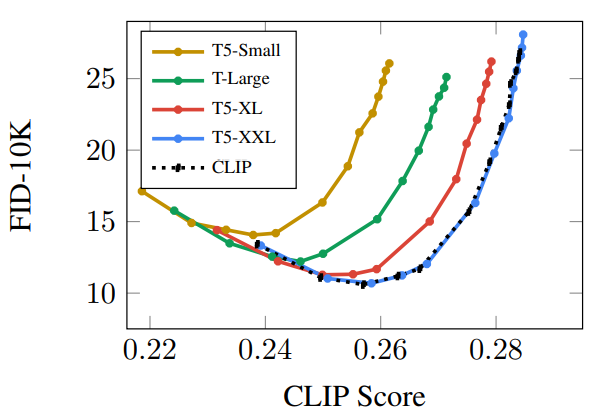
\includegraphics[width=1\textwidth]{images/diffusion_models/stable_diffusion/imagen_clip_score_bigger_llm_encoder.png}
    \end{subfigure}
    \hfill
    \begin{subfigure}[b]{0.7\textwidth}
        \centering
        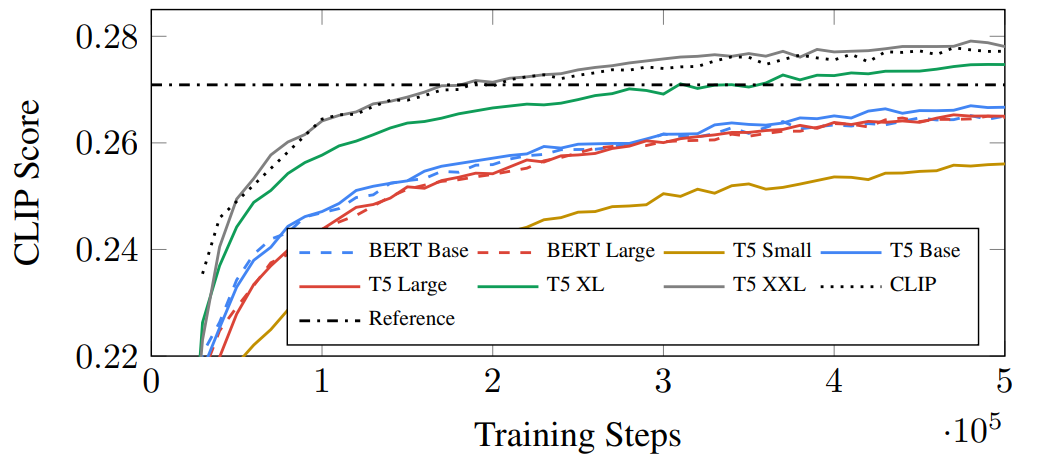
\includegraphics[width=1\textwidth]{images/diffusion_models/stable_diffusion/imagen_clip_score_bigger_llm_encoder2.png}
    \end{subfigure}
    \caption{Imagen paper \cite{imagen} shows that using larger language models as the text encoder (as conditioning mechanism) has more impact on generated image quality than larger image generation components. This is why in Stable Diffusion, the implementation uses CLIP tokenizer instead of BERT tokenizer (which was used in the paper, originally).}
    \label{fig:imagen_clip_score_bigger_llm}
\end{figure}

\begin{figure}[h]
    \centering
    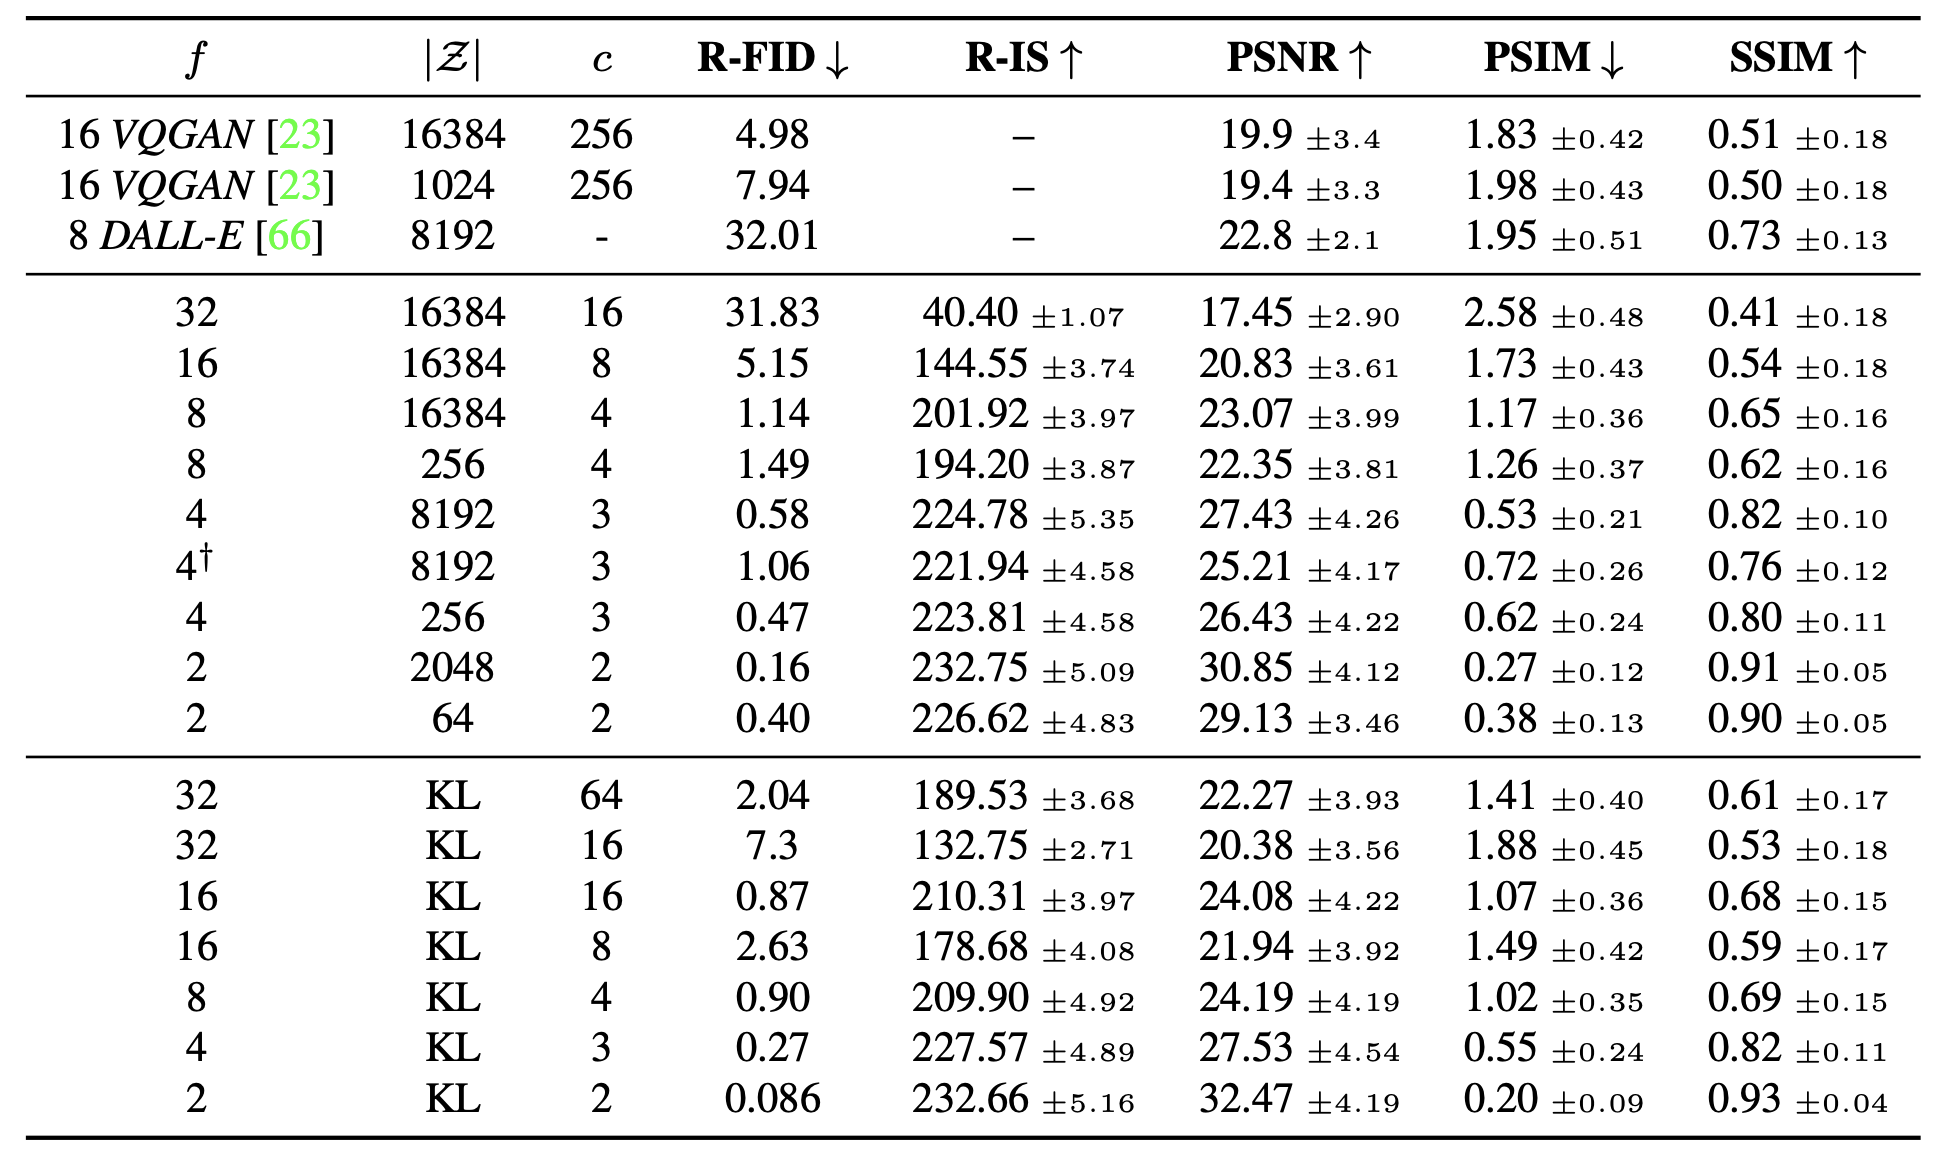
\includegraphics[width=0.8\textwidth]{images/diffusion_models/stable_diffusion/table_8.png}
    \caption{Comparison between VQGAN, DALL-E, and LDM with different amounts of downsampling blocks ($f$), codebook size $|z|$ (or latent representation $z = \varepsilon (x)$ if not VQ-regularized). The less downsampling blocks, the better for LDM in all metrics, however we trade off computation time.}
\end{figure}
